\CHAPTER{The LIGO detector}
\label{chapter2}
%\doublespace

In this chapter I will explain how the LIGO detectors work.

\SECTION{Arms, cavities, etc}

The purpose of the LIGO detectors is to measure the infinitessimal
oscillations of spacetime imparted by far-away astrophysical
processes.  Through clever design and careful engineering, these
machines are capable of resolving these tiny perturbations from the
much louder sea of noise on the surface of the Earth.  \the\columnwidth

As we have seen, a passing gravitational wave modulates the optical
path length of light passing through it, as marked by inertial test
masses.  To exploit this effect and build a detector around it, we
need to arrange to have inertial test masses.  We need to be able to
tell the difference between phase perturbations due to the
gravitational wave and phase perturbations inflicted by our light
source.  We need to eliminate sources of phase variations that would
be louder than the effect we wish to measure.  

\SECTION{A single cavity}

Our first impulse might be to build a single resonant cavity to use as
a gravitational wave detector.  Consider the two-mirror system in
Figure~\ref{fig:fabry-perot}.  By suspending these two mirrors as
pendula, we can simulate intertial test masses.  The resonant optical
cavity is of ubiquitous utility in LIGO, so this discussion will be of
general interest.

Here we will ignore the spatial distribution of light, and its
polarization.  Despite these simplification, the results will have
wide applicability.

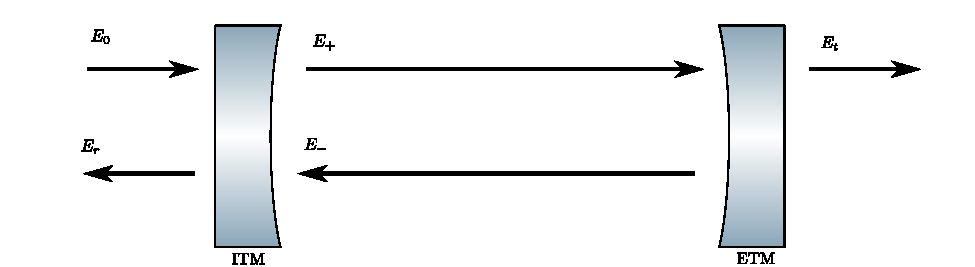
\includegraphics[]{figures/cavity.pdf}

Solving for the fields, we get the amplitude transmission and
reflection coefficients for the cavity:
%
\begin{align}
t_c := & \frac{E_t}{E_0} = 
         \frac{-t_1 t_2 \exp i\phi}
              {1 - r_1 r_2 \exp i2\phi} \\
r_c := & \frac{E_r}{E_0} = 
         \frac{r_1 - \left({r_1}^2 + {t_1}^2\right)r_2 \exp{i2\phi}}
              {1 - r_1 r_2 \exp i2\phi}
\end{align}
%
where $\phi$ is the phase accumulated by the field as it travels from
the first mirror to the second mirror.  The phase depends on both the
laser wavelength and the distance between the mirrors:
$\phi=2\pi(2L/c)\nu$.  The quantity $fsr=c/(2L)$ is the \emph{free
  spectral range}.  It is often useful to write the cavity
reflectivity in the form of a rational transfer function (poles and
zeros):
%
\begin{equation}
r_c(s) = \mathop{\Huge{\Pi}}\limits_{n=-\infty}^{\infty} \frac {s-z_n} {s-p_n}
\end{equation}

For a gravitational wave detector, we might choose $r_2=1$.

We are interested in the phase of the reflected field.  This is easy to find.

\SECTION{A Michelson}
\begin{figure}
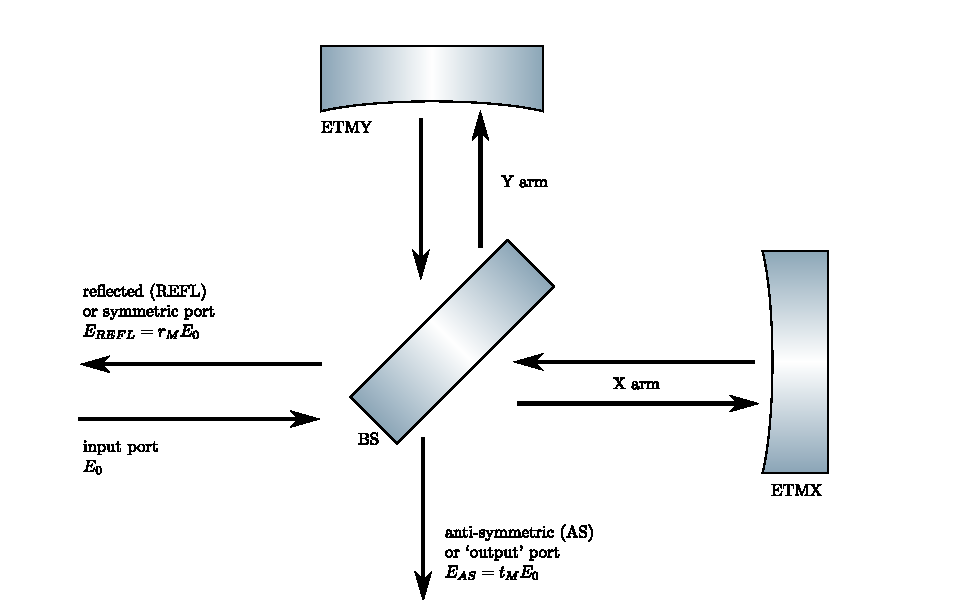
\includegraphics{figures/michelson.pdf}
\caption{\label{fig:michelson}Michelson interferometer}
\end{figure}

By a convenient coincidence, a Michelson interferometer is ideally
suited to gravitational wave detection.  A suitably polarized wave
directly excites the differential mode of the Michelson, while the
Michelson simultaneously provides huge level of common mode noise
rejection.

If we assume a perfect beamsplitter, the transmission and reflection
coefficients for the Michelson are:

\begin{align}
t_M  &= \frac{1}{2}\left(r_x e^{i2\phi_x} - r_y e^{i2\phi_y} \right) \\
r_M  &= \frac{1}{2}\left(r_x e^{i2\phi_x} + r_y e^{i2\phi_y} \right)
\end{align}

Change variables to 
$\phi_- = \phi_x - \phi_y$ and 
$\phi_+ = \phi_x + \phi_y$, i.e. 
%
$\phi_x = (1/2)\left(\phi_+ + \phi_-\right)$
$\phi_y = (1/2)\left(\phi_+ - \phi_-\right)$
which gives
\begin{align}
t_M  &= \frac{1}{2}\left(r_x e^{i2\phi_x} - r_y e^{i2\phi_y} \right) \\
r_M  &= \frac{1}{2}\left(r_x e^{i2\phi_x} + r_y e^{i2\phi_y} \right)
\end{align}

\begin{align}
t_M  &= \frac{1}{2}\left(r_x e^{i\left(\phi_+ + \phi_- \right)} - r_y e^{i\left(\phi_+ - \phi_-\right)} \right) \\
r_M  &= \frac{1}{2}\left(r_x e^{i\left(\phi_+ + \phi_- \right)} + r_y e^{i\left(\phi_+ - \phi_-\right)} \right) 
\end{align}

\begin{align}
t_M  &= \frac{1}{2} e^{i\phi_+} \left(r_x e^{i \phi_- } - r_y e^{-i \phi_-} \right) \\
r_M  &= \frac{1}{2} e^{i\phi_+} \left(r_x e^{i \phi_- } + r_y e^{-i \phi_-} \right) 
\end{align}

Now we can also separate the arm reflectivity into common and differential reflectivity, using $r_x = (1/2)(r_+ + r_-)$ and $r_y = (1/2)(r_+ - r_-)$:

\begin{align}
t_M  &= \frac{1}{2} e^{i\phi_+} \left[ r_+ i \sin \phi_- + r_- \cos \phi_- \right]\\
r_M  &= \frac{1}{2} e^{i\phi_+} \left[ r_+ i \cos \phi_- + r_- \sin \phi_- \right] 
\end{align}

assuming $r_x$ and $r_y$ are real, this leads to:

\begin{align}
P_{AS}   &= \frac{1}{4}\left( {r_+}^2 \sin^2 \phi_- + {r_-}^2 \cos^2 \phi_-\right) \\
P_{REFL} &= \frac{1}{4}\left( {r_+}^2 \cos^2 \phi_- + {r_-}^2 \sin^2 \phi_-\right) \\
\end{align}

\cite{Fritschel2001Readout}
\SECTION{Power recycling}

The Michelson interferometer tuned to a dark fringe for the laser
carrier sends most of the laser power back towards the laser.  Instead
of discarding this power, it can be sent back into the Faby-Perot
Michelson interferometer.  This is done by adding an additional
mirror, the \emph{power recycling mirror}, that forms a resonant
cavity with the rest of the interferometer.  Choosing the reflectivity
of the power recycling mirror to match the effective reflectivity of
the rest of the interferometer makes this cavity critically coupled;
ideally all of the laser carrier is coupled into the interferometer
and very little is reflected.  Most of the light stays in the
interferometer until it is lost to scattering or absorption.

\SECTION{Interferometer Sensing and Control}

The laser light incident on the interferometer is phase-modulated at
several frequencies, producing optical sidebands on the laser carrier.
Light extracted from the interferometer at its various ports is
incident on photodiodes; the photodiode signals are demodulated to
produce signals.


\SECTION{LIGO}
Construction began on the LIGO observatories in YEAR.  After many
years of commissioning, the detectors reached their design sensitivity
in YEAR.  Having met the conditions described in the science
requirements document, LIGO commenced a long observational run,
accumulating one year of coincident data over a period of two calendar
years.

\SECTION{Summary of changes made for Enhanced LIGO}

After the successful completion of the Initial LIGO science goals, it
was decided
\cite{Adhikari2006Enhanced,T050252,JoshSmithEnhancedAdvanced} to
attempt to further improve the detector sensitivity by aggressively
implementing a few prototype Advanced LIGO technologies.

Changes included:
\begin{itemize}
\item Fancy new laser
\item Renovation of the input optics to handle higher power operation, including new electro-optic modulators \cite{Quetschke2008ElectroOptic}
\item Installation of an output mode cleaner, supported by a prototype of the advanced LIGO in-vacuum seismic isolation system
\item New Thermal Compensation System to handle the higher power
\end{itemize}

DC readout has been implemented previously at the Caltech 40 meter
prototype \cite{Ward2008DC,RobWardThesis} and the GEO 600
detector\cite{GeoDC,Prijatelj2010,Degallaix2010Commissioning}.  The
current configuration of Virgo incorporates an output mode cleaner but
uses RF heterodyne readout\cite{Acernese2008Virgo}.

\SECTION{History of the noise during Enhanced LIGO}

\SECTION{Future directions}

